% DOI for EIDORS v3.13 ?  10.5281/zenodo.19702479
% DOI for slides 10.5281/zenodo.19702540
\documentclass[10pt,a4paper]{article}
% ========================== DO NOT MODIFY =================================== %
\usepackage[a4paper,left=2.0cm,top=2.0cm,right=2.0cm,bottom=2.0cm]{geometry}
\usepackage{amssymb,amsmath} % If amsmath is required
\usepackage[implicit=false]{hyperref}
\usepackage[utf8]{inputenc}
\usepackage[T1]{fontenc}
\usepackage{mathptmx}  % Replaced obsolete times package; defines Times Roman as default font
\usepackage{multicol}
\usepackage{amssymb,amsmath} % If amsmath is required
\usepackage{graphicx}
\usepackage{booktabs}
\usepackage{titling}
\usepackage{authblk} % Formats affiliation section
\usepackage{float}
\usepackage{enumitem}
\usepackage{siunitx}
\usepackage{xcolor}

\def\xH/{\hat{\mathbf{x}}}
\def\JB/{\mathbf{J}}
\def\yB/{\mathbf{y}}
\def\vB/{\mathbf{v}}
\usepackage{bm} % bold Greek
\def\SG/{\bm{Sigma}}
\def\RB/{\mathbf{R}}

\newcommand{\ConferenceName}{26\textsuperscript{th} International Conference on Biomedical Applications of Electrical Impedance Tomography (EIT 2026), Sheffield, UK}
\def\xH/{\hat{\mathbf{x}}}
\def\JB/{\mathbf{J}}
\def\yB/{\mathbf{y}}
\def\vB/{\mathbf{v}}
\usepackage{bm} % bold Greek
\def\SG/{\bm{Sigma}}
\usepackage{hyperref}
\hypersetup{
    colorlinks=true,
    linkcolor=blue,
    filecolor=blue,      
    urlcolor=blue,
}
    
\usepackage{fancyhdr}
\fancyhf{}
\setlength{\headheight}{3em}
\pagestyle{fancy}
\renewcommand{\headrulewidth}{0pt} % Remove underline in header

\fancypagestyle{firstpage}
{
  \chead{\footnotesize{\ConferenceName}}
}

\usepackage[small,compact]{titlesec}
% Can be used to adjust spacing between Abstract section and Introduction section
	%{0pt}  % Left margin indentation
	%{5pt}  % Space before the section title
	%{3pt}  % Space after the section title (before text)
\titlespacing*{\section}{0pt}{8pt}{2pt}  
\titlespacing*{\subsection}{0pt}{6pt}{2pt}
\titlespacing*{\subsubsection}{0pt}{3pt}{-1pt}

\usepackage[numbers,sort&compress]{natbib}
\usepackage[small,bf,tableposition=top,figureposition=bottom,skip=2pt]{caption}

% Limit space between floats and text
\setlength{\textfloatsep}{10pt plus 1.0pt minus 2.0pt}
% Shrink the list environments
\setlist{noitemsep}
\setlist{nolistsep}

% Format of the front matter
\renewcommand{\Affilfont}{\small}
\setlength{\affilsep}{1ex}
\renewcommand\Authands{, }
\setlength{\droptitle}{-2cm}


% Shrink the bibliography
\let\oldthebibliography=\thebibliography
\let\endoldthebibliography=\endthebibliography
\renewenvironment{thebibliography}[1]{%
\begin{oldthebibliography}{#1}%
	\setlength{\parskip}{0ex}%
	\setlength{\itemsep}{0ex}%
}
{
	\end{oldthebibliography}%
}

% Document macros
\newcommand{\etal}{\textit{et al}.} % Make et al. italic throughout the text
\renewcommand*{\figurename}{Fig.} % Set the shorter form for figures caption
\renewcommand*{\tablename}{Tab.} % Set the shorter form for tables caption

% ========================== DO NOT MODIFY =================================== %


% ============================================================================ %
% ========================== USER SECTION ==================================== %
%------------------------------- FRONT MATTER -------------------------------- %

\newcommand{\PresentingAuthor}{Andy Adler}
\newcommand{\DocumentTitle}{EIDORS v3.13}

%% PDF meta data:
\hypersetup{ % more settings like bookmarks true/false are defined in section \usepackage
	pdfauthor={\PresentingAuthor},
	pdftitle={\DocumentTitle},
	pdfsubject={\ConferenceName},
	pdfkeywords={EIT2026}
}


\title{\DocumentTitle
\vspace{-1.5ex}} % Remove vertical space

\author[1]{\PresentingAuthor}

\affil[1]{Systems and Computer Engineering, Carleton University, Ottawa, Canada, \protect\href{mailto:adler@sce.carleton.ca}{\underline{adler@sce.carleton.ca}}}
\date{} % Keep it empty to remove date field
%----------------------------------------------------------------------------- %


\begin{document}
\maketitle
\thispagestyle{firstpage}
\vspace{-1.5cm}
\begin{multicols}{2}

\noindent {\bf Abstract:}
This paper announces the release of version 3.13 of the
EIDORS software suite. We review its new features, and 
make available suitable EIT illustrations.

\section{Introduction}

We proudly announce the release of EIDORS version 3.13,
for the 26th Int.\ Conf.\ on Biomedical Applications of EIT,
in July 2026.
The software is available at \href{www.eidors.org}{eidors.org}\, and licensed under the GNU GPLv2 or GPLv3. Archived versions are available on Zenodo
\cite{eidors3p13, eidors3p12,
      eidors3p11,
      eidors3p10,
      eidors3p9p1,
      eidors3p9,
      eidors3p8}, and all versions available on 
\href{www.sourceforge.net}{sourceforge.net}
\cite{adler2005, adler2006, adler2008}.


EIDORS provides free software algorithms for forward modelling
and inverse solutions
of Electrical Impedance and (to some extent) Diffusion-based Optical Tomography, in
medical, industrial and geophysical settings.
EIDORS also aims to share data and promote
collaboration.

\section{Features and Growth}
Release 3.13 of EIDORS builds upon a strong foundation in reconstruction
algorithms, adding and improving a number of aspects.
\begin{itemize}
\item improved / less fragile netgen interface
\item refactored extruded mesh shapes
\item support for acousto-electric tomography
\item improved documentation
\item graphcs improvements and bug work-arounds
\item support for new vendor file formats
\item better octave support

\item (As always) speed-ups and bug fixes 
\end{itemize}

EIDORS-related citations continue to grow (table~1).  %table~\ref{tbl:cite}.

\noindent
In conclusion, EIDORS version 3.13 (hopefully) continues to be useful.

\begin{table}[H]
  \footnotesize
\centering
%From: http://amath.colorado.edu/documentation/LaTeX/reference/tables/ex1.html
\caption{EIDORS Citations
 (Apr 2026, scholar.google.com).
}
\label{tbl:cite}
\begin{tabular}{r@{\hspace{1mm}}lcr}
  \toprule
  & Paper & Date & \hspace{-2mm}Citations \\
  %{@{\extracolsep{\fill}}@{}|c|ccc|r|}
  \midrule
  \cite{vauhkonen2001} & A MATLAB package for the EIDORS project \ldots\hspace{-5mm}  
    & 2001 & 370 \\
  \cite{polydorides2002phd} & Image reconstruction algorithms for \ldots
    & 2002 & 211 \\
  \cite{polydorides2002matlab} & A Matlab toolkit for three-dimensional \ldots
    & 2002 & 613 \\
  \cite{adler2005} & EIDORS: Towards a community-based \ldots
    & 2005 & 53 \\
  \cite{adler2006} & Uses and abuses of {EIDORS}: An extensible \ldots
    & 2006 & 1109 \\
  \cite{adler2008} & Simple FEMs aren't as good as we thought \ldots
    & 2008 &  26 \\
  \cite{eidors3p9} & EIDORS version 3.9
    & 2017 & 40 \\
  \cite{eidors3p10} & EIDORS version 3.10
    & 2019 & 9 \\
  \bottomrule
\end{tabular}
\vspace{-1em}
\end{table}

\begin{figure}[H]
  \vspace{-2.5mm}
\centering
% trim=left botm right top
 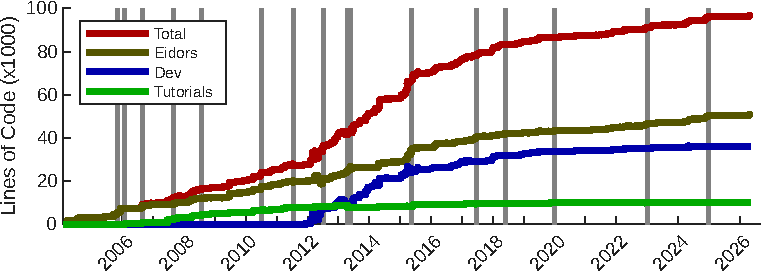
\includegraphics[width=.99\columnwidth]{fig_loc.pdf}
\caption{%
%graph and table combo chart, including line for test code.
  Lines of Code (LoC) in Matlab files in the EIDORS code-base vs.\ time; Total
   (red), EIDORS (i.e.\ release branch, brown), Tutorials (green), development code (blue).
   Releases are indicated by gray bars (The 3.12 release is
   at the right).
}
\label{fig:loc}
\end{figure}

\section{EIT Illustrations}

We make available software and illustrations of the basic
concepts of EIT.
Software is available in {\tt eidors/examples/eit\_intro} and
figures at \href{https://doi.org/10.5281/zenodo.19702540}
                            {DOI:10.5281/zenodo.19702540}, 
under an creative commons license for
use in papers and presentations (fig~\ref{fig:illustrations}).

Illustrations of equipotential backprojection are often used
to illustrate ``how EIT works'', even though this 
is no longer used in any clinical or research EIT systems.

However, it is possible to illustrate linearized time-difference EIT image reconstruction
in this way (Fig~\ref{fig:illustrations}C).
From a solution $\xH/$ which minimizes:
$\| \xH/ - \JB/ \yB/ \|$
for sensitivity matrix $\JB/$ and difference data $\yB/$,
$\xH/ =
 ( \JB/^T  \JB/^T + \RB/ )^{-1} 
\JB/^T
 \yB/ = (\mbox{Filter})(\mbox{Backprojection})\yB/
$


\begin{figure}[H]
  \vspace{-2.5mm}
\centering
 \includegraphics[page=2,width=.6\columnwidth]{figures-EIDORS-v3.13.pdf}
\put(-184,45){\bf (A)}

 \includegraphics[page=3,width=.99\columnwidth]{figures-EIDORS-v3.13.pdf}
\put(-230,95){\bf (B)}

\vspace{2mm}
\raisebox{9mm}{\includegraphics[page=4,width=.4\columnwidth]{figures-EIDORS-v3.13.pdf}}
 \includegraphics[page=16,width=.59\columnwidth]{figures-EIDORS-v3.13.pdf}%
\put(-230,90){\bf (C)}%
\put(-130,90){\bf (D)}%
\caption{%
EIT Illustrations
 (Images and data from \cite{heinrich2006}):
(A) Subject and FEM;
(B) adjacent-drive measurement and the equipotential lines
associated with a change in heart blood volume;
(C) EIT image from four most sensitive measurements of the heart region;
(D) EIT images and waveforms of breathing and heart activity.
}
\label{fig:illustrations}
\end{figure}
\vspace{-5mm}




\footnotesize
\begin{thebibliography}{}
\bibitem{eidors3p13}
   Adler, ``EIDORS v3.13'',
\href{http://dx.doi.org/10.5281/zenodo.19702479}{Conf EIT 2026}, Sheffield, UK.

\bibitem{eidors3p12}
   Adler, Grychtol, ``EIDORS v3.12'',
\href{http://dx.doi.org/10.5281/zenodo.13316995}{Conf EIT 2024}, Hangzhou, China.
\bibitem{eidors3p11}
   Adler, ``EIDORS v3.11'',
\href{http://dx.doi.org/10.5281/zenodo.7495740}{Conf EIT 2022}, Seoul, S~Korea.

\bibitem{eidors3p10}
   Adler, ``EIDORS v3.10'',
   \href{http://dx.doi.org/10.5281/zenodo.3247168}{Conf EIT 2019}, London, UK.

\bibitem{eidors3p9p1}
   Adler {\em et\,al},\,``EIDORS v3.9.1'',\,%
   \href{http://dx.doi.org/10.5281/zenodo.1257670}{DOI:zenodo.1257670},\,%
    2018.

\bibitem{eidors3p9}
   Adler {\em et\,al}, ``EIDORS v3.9'',
   \href{http://dx.doi.org/10.5281/zenodo.583266}{Conf EIT 2017}, Neuchâtel, Suisse.

%\bibitem{adler2017}
%Adler A {\em et\,al}, % Andy Adler, Alistair Boyle, Fabian Braun, Michael G. Crabb, Bartłomiej Grychtol, William R. B. Lionheart, Henry F. J. Tregidgo, Rebecca Yerworth
%\href{https://zenodo.org/record/557093}{\em Proc EIT2017}, p.63, 
%Dartmouth, NH, USA,  2017.

\bibitem{eidors3p8}
   Adler {\em et\,al}, ``EIDORS v3.8'',
   \href{http://dx.doi.org/10.5281/zenodo.17559}{Conf EIT 2015}, Dartmouth, NH, USA.

\bibitem{adler2008}
Adler, Borsic {\em et\,al},
%Simple FEMs aren't as good as we \ldots
{\em Proc EIT2008}, Hannover, NH, USA, 2008.

%\bibitem{adler2015}
%Adler A {\em et\,al}, %Alistair Boyle, Michael G Crabb, Hervé Gagnon, Bartłomiej Grychtol, Nolwenn Lesparre, William R.B. Lionheart,
%\href{https://zenodo.org/record/17752}{\em Proc EIT2015}, p.19, 
% Neuchâtel, Switzerland, 2015.

\bibitem{adler2005}
Adler, Lionheart,
%"EIDORS: Towards a community-based extensible software base for EIT." 6th Conference on Biomedical Applications of Electrical Impedance Tomography, London, UK. 2005.
{\em Proc EIT2005}, London, UK, 2005.

%
\bibitem{adler2006}
Adler, Lionheart,
{\em Physiol Meas} 27:S25--S42, 2006.

\bibitem{heinrich2006}
Heinrich {\em et\,al} Int Car Med, 32:1392-1398, 2006.
%S. Heinrich, H. Schiffmann, A. Frerichs, A. Klockgether-Radke, I. Frerichs, Body and head position effects on regional lung ventilation in infants: an electrical impedance tomography study. Intensive Care Med., 32:1392-1398, 2006.

\bibitem{polydorides2002phd}
   Polydorides,
%{\em Image Reconstruction Algorithms for Soft-Field Tomography},
 {\em Ph.D. thesis}, U Manchester, UK, 2002.
\bibitem{polydorides2002matlab}
   Polydorides N, Lionheart, % WRB,
   {\em Meas Sci Tech}, 13:1871--1883, 2002.

\bibitem{vauhkonen2001}
   Vauhkonen  {\em  et\,al},
%  Vauhkonen \& M, Lionheart WRB {\em  et\,al},
   {\em  Physiol Meas}, 22:107--111, 2001.

\end{thebibliography}
\end{multicols}


\end{document}
